\section{Applications of Differentiation}

\subsection{Revision}

%<*sec:diffrev>
\begin{Exercise}[label={\thesubsection.\the\value{Exercise}}]
Find  $f'(x)$ for
	\multicolq{
	\Question $\displaystyle f(x) = 6 x^3$
	\Question $\displaystyle f(x) = \frac{9}{x^4} $
	\Question $\displaystyle f(x) = 5 x^5  + 4 x^2 + 7$
	}
\end{Exercise}
\begin{Answer}[ref=\ExerciseLabel]
\multicolq{
	\Question $\displaystyle 18 x^2$
	\Question $\displaystyle -\frac{36}{x^5}$
	\Question $\displaystyle 25 x^4 + 8x$
	}
\end{Answer}

\begin{Exercise}[label={\thesubsection.\the\value{Exercise}}]
Find  $s'(t)$ for $s(t) = - 5 t^2 + 10 t + 25$
\end{Exercise}
\begin{Answer}[ref=\ExerciseLabel]
$-10 t + 10$
\end{Answer}


\begin{Exercise}[label={\thesubsection.\the\value{Exercise}}]
Find  $f'(x)$ for
	\multicolq{
	\Question $\displaystyle f(x) = (x^3 + 3x)^6$
	\Question $\displaystyle f(x) = e^{4x^2 - 3x} $
	\Question $\displaystyle f(x) = \cos(5x+3)$
	}
\end{Exercise}
\begin{Answer}[ref=\ExerciseLabel]
\multicolq{
	\Question $\displaystyle 6(3x^2 + 3)(x^3 + 3x)^5$
	\Question $\displaystyle (8x - 3) e^{4x^2-3x}$
	\Question $\displaystyle - 5 \sin (5x + 3)$
	}
\end{Answer}

\begin{Exercise}[label={\thesubsection.\the\value{Exercise}}]
Find  $f'(x)$ for
	\multicolq{
	\Question $\displaystyle f(x) = 2x^2 \ln (3 x^3)$
	\Question $\displaystyle f(x) =  6 x^3 e^{x}$
	\Question $\displaystyle f(x) = \sin(x)\cos(x)$
	}
\end{Exercise}
\begin{Answer}[ref=\ExerciseLabel]
\multicolq{
	\Question $\displaystyle 4x\ln (3x^3) + 6x$
	\Question $\displaystyle 18x^2e^x + 6x^3 e^x$
	\Question $\displaystyle \cos^2(x)  - \sin^2(x) $
	}
\end{Answer}

\begin{Exercise}[label={\thesubsection.\the\value{Exercise}}]
Find  $f'(x)$ for
	\multicolq{
	\Question $\displaystyle f(x) = \frac{3x}{x - 3} $
	\Question $\displaystyle f(x) = \frac{x^2}{1 + e^{x}}$
	\Question $\displaystyle f(x) = \tan(x)$
	}
\end{Exercise}
\begin{Answer}[ref=\ExerciseLabel]
\multicolq{
	\Question $\displaystyle -\frac{9}{(x-3)^{2}} $
	\Question $\displaystyle \frac{(2x)(1 + e^x) - (x^2)(e^x)}{(1 + e^x)^{2}}$
	\Question $\displaystyle \frac{1}{\cos^2(x)}$
	}
\end{Answer}
%</sec:diffrev>

\subsection{Linear Approximation}

%<*sec:difflinear>
\begin{Exercise}[label={\thesubsection.\the\value{Exercise}}]
Find the linear approximation of the function $\cos(x)$ for $x$ near $\frac{\pi}{2}$.
\end{Exercise}
\begin{Answer}[ref=\ExerciseLabel]
$\displaystyle \frac{\pi}{2}-x$
\end{Answer}

\begin{Exercise}[label={\thesubsection.\the\value{Exercise}}]
Find the linear approximation of the function $x^3 + \ln(x)$ for $x$ near $2$.
\end{Exercise}
\begin{Answer}[ref=\ExerciseLabel]
$\displaystyle \ln(2) - 17 + 12.5 x$
\end{Answer}

\begin{Exercise}[label={\thesubsection.\the\value{Exercise}}]
 The radius of a (spherical) star was $r=a$ and was observed to increase by 0.01\%. Use linear approximation to estimate the percentage its surface area increases by.
\end{Exercise}
\begin{Answer}[ref=\ExerciseLabel]
$0.02\%$ 
\end{Answer}

\begin{Exercise}[label={\thesubsection.\the\value{Exercise}}]
Estimate the values $\sqrt{82}$ and $\sqrt{80}$ using linear approximation. How good are these approximations? \newline
\emph{Hint: set $f(x)=\sqrt{x}$ and $a=81$.}
\end{Exercise}
\begin{Answer}[ref=\ExerciseLabel]
$\displaystyle 9+\frac{1}{18}, 9-\frac{1}{18}$ 
\end{Answer}

\begin{Exercise}[label={\thesubsection.\the\value{Exercise}}]
 A $100$m long pipe of diameter 4m is covered by insulation $h$m thick and then buried underground in soil. Use linear approximation to estimate how much extra soil is displaced by the insulation.
\end{Exercise}
\begin{Answer}[ref=\ExerciseLabel]
$\displaystyle 400\pi h$ m$^3$ 
\end{Answer}

\begin{Exercise}[label={\thesubsection.\the\value{Exercise}}]
To keep costs down in the previous question we are only allowed to displace an extra 100m$^3$ of soil by adding the insulation. Use linear approximation to estimate the maximum thickness allowable.
\end{Exercise}
\begin{Answer}[ref=\ExerciseLabel]
$\displaystyle h \approx \frac{1}{4\pi} \approx 0.0796$m.
\end{Answer}

\begin{Exercise}[label={\thesubsection.\the\value{Exercise}}]
The restoring force on a pendulum is given by $F = - m g \sin \theta$. For the case $m = 1$kg, $g = 10 m s^{-2}$ and $\theta = 0.1$ radians, determine $F$ using 1) the formula and 2) when the small angle approximation for $\sin(\theta)$ is applied.
\end{Exercise}
\begin{Answer}[ref=\ExerciseLabel]
$-0.998$ and $-1 $ 
\end{Answer}
%</sec:difflinear>



\subsection{Maclaurin Series}

%<*sec:diffmac>
\begin{Exercise}[label={\thesubsection.\the\value{Exercise}}]
Find the $2$nd-degree Maclaurin polynomial for $\sqrt{1+x}$.
\end{Exercise}
\begin{Answer}[ref=\ExerciseLabel]
$\displaystyle 1 + \frac{ x}{2} - \frac{x^2}{8}$ 
\end{Answer}


\begin{Exercise}[label={\thesubsection.\the\value{Exercise}}]
Find $3$rd-degree Maclaurin polynomial for $\ln(1+x)$.
\end{Exercise}
\begin{Answer}[ref=\ExerciseLabel]
$\displaystyle x - \frac{ x^2}{2} + \frac{x^3}{3}$  
\end{Answer}

\begin{Exercise}[label={\thesubsection.\the\value{Exercise}}]
Find $4$th-degree Maclaurin polynomial for $\cos(x)$.
\end{Exercise}
\begin{Answer}[ref=\ExerciseLabel]
$\displaystyle 1 - \frac{ x^2}{2} + \frac{x^4}{24}$
\end{Answer}

\begin{Exercise}[label={\thesubsection.\the\value{Exercise}}]
Find $2$nd-degree Maclaurin polynomial for $\ln\left(1 + e^x\right)$.
\end{Exercise}
\begin{Answer}[ref=\ExerciseLabel]
$\displaystyle \ln(2) + \frac{ x}{2} + \frac{x^2}{8}$ 
\end{Answer}
%</sec:diffmac>

\subsection{Taylor Series}

%<*sec:difftay>

\begin{Exercise}[label={\thesubsection.\the\value{Exercise}}]
Find $3$rd-degree Taylor polynomial expansion of $\cos(x)$ for $x$ near $\frac{\pi}{2}$.
\end{Exercise}
\begin{Answer}[ref=\ExerciseLabel]
$\displaystyle -\left(x-\frac{\pi}{2}\right) + \frac{1}{6}\left(x-\frac{\pi}{2}\right)^3$ 
\end{Answer}


\begin{Exercise}[label={\thesubsection.\the\value{Exercise}}]
Find $3$rd-degree Taylor polynomial expansion of $\ln(x)$ about $x = 1$.
\end{Exercise}
\begin{Answer}[ref=\ExerciseLabel]
$\displaystyle (x-1) - \frac{1}{2}(x-1)^2 + \frac{1}{3}(x-1)^3$
\end{Answer}
%</sec:difftay>


\subsection{Optimisation}

%<*sec:diffopp>
\begin{Exercise}[label={\thesubsection.\the\value{Exercise}}]
A variable rectangle has a constant area of $49$.  Find the lengths of the sides when the perimeter is a minimum.
\end{Exercise}
\begin{Answer}[ref=\ExerciseLabel]
$7$ by $7$
\end{Answer}

\begin{Exercise}[label={\thesubsection.\the\value{Exercise}}]
A rectangular block has a square base.  Its total surface area is $150$.
\Question If the base length is $x$ , show that the volume $V$ of the block is $\displaystyle V = \frac{75x -x^3}{2}$
\Question Find the dimensions of the block if the volume is a maximum.
\end{Exercise}
\begin{Answer}[ref=\ExerciseLabel]
\multicolq[2]{
\Question {(Proof required)}
\Question $5$ by $5$ by $5$ 
}
\end{Answer}

\begin{Exercise}[label={\thesubsection.\the\value{Exercise}}]
An open box is to be made with a square base. The volume of the box is 32 cm$^3$. Find the dimensions of the box if the surface area of the box is a minimum.
\end{Exercise}
\begin{Answer}[ref=\ExerciseLabel]
$4$ by $4$ by $2$
\end{Answer}

\begin{Exercise}[label={\thesubsection.\the\value{Exercise}}]
A rectangular box-shaped house is to have a square floor.  Four times as much heat per square metre is lost through the roof as through the walls: no heat is lost through the floor. The house has to enclose $2000$ cubic metres.  Find the dimensions of the house so as to minimise heat loss.
\end{Exercise}
\begin{Answer}[ref=\ExerciseLabel]
$10$ by $10$ by $20$
\end{Answer}

\begin{Exercise}[label={\thesubsection.\the\value{Exercise}}]
A rectangular field is to be fenced off along a road.  The fence along the road costs 3 pounds per metre while on the other sides it costs $2$ pounds per metre.  Calculate the maximum area that can be fenced off for $400$ pounds.
\end{Exercise}
\begin{Answer}[ref=\ExerciseLabel]
$2000$
\end{Answer}

\begin{Exercise}[label={\thesubsection.\the\value{Exercise}}]
The cost per hour of running a train is given by $k\left(100 + \frac{v^2}{36}\right)$ where $k$ is a positive constant and $v$ (in mph) is the average speed of the journey. Find the speed $v$ that makes the trip from Edinburgh to London cheapest, assuming that the distance is 400 miles.
\end{Exercise}
\begin{Answer}[ref=\ExerciseLabel]
$60$mph 
\end{Answer}

\begin{Exercise}[label={\thesubsection.\the\value{Exercise}}]
During essential maintenance work, an average speed limit is imposed in the previous question and the maximum average speed allowed is $v=50$ mph. Find the optimal speed for the cheapest trip in this case.
\end{Exercise}
\begin{Answer}[ref=\ExerciseLabel]
$50$mph 
\end{Answer}

\begin{Exercise}[label={\thesubsection.\the\value{Exercise}}]
The price $P$ (in \pounds) that a specialised component can be sold for depends on the average number $x$ manufactured each day. Note that the average number $x$ need not be a whole number. The process requires at least 1 to be made each day, and there is capacity to make up to 10.
The relationship between price and average number per day is found to be
\begin{equation*}
     P(x) = 500 - x^3 - 72 x + 15 x^2.
\end{equation*}
The turning points of this function are at $x=4,6$. Use the second derivative test on each to determine if it is a local maximum or minimum.
State the allowable range for $x$, find the values of $x$ where the global maximum and minimum occur and state clearly what the global maximum and minimum prices are. 
\end{Exercise}
\begin{Answer}[ref=\ExerciseLabel]
Local: Min $x=4$, Max $x=6$. $1 \leq x \leq 10$. Global: Max $x=1$, Min$x=10$.
\end{Answer}
%</sec:diffopp>

\subsection{Solution to Differential Equations}

%<*sec:diffdiffeq>
\begin{Exercise}[label={\thesubsection.\the\value{Exercise}}]
In a certain chemical reaction, the concentration $y(t)$ of a substance is deceasing at a rate proportional to the square of its value at that instant. Obtain the differential equation satisfied by $y(t)$ using $ k > 0 $ is the constant of proportionality. 
\end{Exercise}
\begin{Answer}[ref=\ExerciseLabel]
$\frac{dy}{dt} = -ky^2$
\end{Answer}

\begin{Exercise}[label={\thesubsection.\the\value{Exercise}}]
For a constant $C$, verify that $y = 2 + \frac{C}{t}$ is a solution of 
\begin{equation*}
t \frac{dy}{dt} +y = 2
\end{equation*}
Hence find the solution with $y=7$ when $t=3$.
\end{Exercise}
\begin{Answer}[ref=\ExerciseLabel]
Particular solution: $y = 2 + \frac{15}{t}$
\end{Answer}

\begin{Exercise}[label={\thesubsection.\the\value{Exercise}}]
The velocity $y(t)$ of a particle moving in a resisting medium satisfies the differential equation
\begin{equation*}
\frac{dy}{dt} = -t -y
\end{equation*}
Verify that the solution with $y(0) = 5$ is $y(t) = 1-t +4e^{-t}$.   
\end{Exercise}

\begin{Exercise}[label={\thesubsection.\the\value{Exercise}}]
The height $y(t)$ of a tank of water which is being drained satisfies the differential equation $y'(t) = -16 \sqrt{y(t)}$.  Verify that the solution with $y(0) = 1$ is $y(t) = (1-8t)^2$.
\end{Exercise}


\begin{Exercise}[label={\thesubsection.\the\value{Exercise}}]
In an electric circuit, the current $\,y(t)\,$ satisfies the differential equation 
\begin{equation*}
\frac{dy}{dt} = E -y
\end{equation*}
where the applied voltage $E$ is a constant.  Verify that the solution with $y(0) = 0$ is $y(t) = E(1 - e^{-t})$.  What is the value of the current for large $t$?
\end{Exercise}
\begin{Answer}[ref=\ExerciseLabel]
$y(t) \rightarrow E$ as $t$ gets large.
\end{Answer}

\begin{Exercise}[label={\thesubsection.\the\value{Exercise}}]
A hard-boiled egg is put in a basin of water whose temperature is $18^{\circ}C$.  The temperature of the egg at time $t$ is  $y(t)$, and $y(t)$ is decreasing at a rate proportional to $y(t) -18$. Let $k > 0$ be the constant of proportionality. Obtain the differential equation satisfied by $y(t)$. Verify that $y(t) = 18 + Ce^{-kt}$ is a solution where $C$ is a constant. Hence find $y(t)$ if the initial temperature of the egg  is $98^{\circ} C\,$.
\end{Exercise}
\begin{Answer}[ref=\ExerciseLabel]
$\frac{dy}{dt} = -k(y-18)$ and $y(t) = 18+ 80e^{-kt}$
\end{Answer}

\begin{Exercise}[label={\thesubsection.\the\value{Exercise}}]
Verify that $y = t \ln(t) +Ct$ is a solution of
\begin{equation*}
t \frac{dy}{dt} = t+y
\end{equation*}
where $C$ is a constant.  Hence find the solution with $y=5$ when $t=1$.
\end{Exercise}
\begin{Answer}[ref=\ExerciseLabel]
$y(t) = t\ln(t) + 5t$
\end{Answer}

\begin{Exercise}[label={\thesubsection.\the\value{Exercise}}]
Verify that $y(t) = A \sin(2t) + B \cos(2t)$ is a solution of 
\begin{equation*}
\frac{d^2 y}{dt^2} = -4 y
\end{equation*}
for all choices of $A$ and $B$. Find the values of $A$ and $B$ to satisfy the initial conditions $y(0) = 7$, $y'(0)=-3$.
\end{Exercise}
\begin{Answer}[ref=\ExerciseLabel]
$A=-\frac{3}{2}$, $B=7$
\end{Answer}
%</sec:diffdiffeq>

\section{Techniques of Integration}

\subsection{Revision of Integration}

%<*sec:techintrev>
\begin{Exercise}[label={\thesubsection.\the\value{Exercise}}]
Evaluate the following:
\multicolq{
\Question $\displaystyle \int 2 x^3 - 16 x \, dx$
\Question $\displaystyle \int (e^\alpha + 3) \, d\alpha$
\Question $\displaystyle \int -x^{\frac{3}{2}} \, dx$
}
\end{Exercise}
\begin{Answer}[ref=\ExerciseLabel]
\multicolq{
\Question $\displaystyle \frac{1}{2} x^4 - 8 x^2 + C$
\Question $\displaystyle e^{\alpha} + 3 \alpha +C $
\Question $\displaystyle -\frac{2}{5} x^{\frac{5}{2}} + C$
}
\end{Answer}

\begin{Exercise}[label={\thesubsection.\the\value{Exercise}}]
Evaluate the following:
\multicolq{
\Question $\displaystyle \int_1^2  4 x^3 - 2 x \, dx$
\Question $\displaystyle \int_\pi^{2 \pi} \sin(\theta) \, d\theta$
\Question $\displaystyle \int_1^4 \frac{1}{2x} dx$
}
\end{Exercise}
\begin{Answer}[ref=\ExerciseLabel]
\multicolq{
\Question $12$
\Question $-2$
\Question $\ln(2)$
}
\end{Answer}

\begin{Exercise}[label={\thesubsection.\the\value{Exercise}}]
Evaluate $\displaystyle \int_1^\infty \frac{1}{x^2} \, dx$
\end{Exercise}
\begin{Answer}[ref=\ExerciseLabel]
$1$
\end{Answer}
%</sec:techintrev>

\subsection{Partial Fractions}

%<*sec:techintpartial>
\begin{Exercise}[label={\thesubsection.\the\value{Exercise}}]
Use partial fractions to find  the integrals below.
\multicolq{
\Question $\displaystyle \int \frac{1}{(2+2x)(x-3)}\; dx$
\Question $\displaystyle \int \frac{13x-4}{6x^2-x-2}\; dx$
\Question $\displaystyle \int \frac{1}{x^2-2x-3}\; dx$
}
\end{Exercise}
\begin{Answer}[ref=\ExerciseLabel]
\multicolq[2]{
\Question $\displaystyle -\frac{1}{8}\ln(2+2x)+\frac{1}{8} \ln(x-3)+C$
\Question $\displaystyle \frac{3}{2}\ln(2x+1)+\frac{2}{3}\ln(3x-2)+C$
\Question $\displaystyle -\frac{1}{4}\ln (1+x)+\frac{1}{4}\ln (x-3)+C$
}
\end{Answer}

\begin{Exercise}[label={\thesubsection.\the\value{Exercise}}]
Evaluate the following integrals.
\multicolq{
\Question $\displaystyle \int_1^2 \frac{1}{(1+x)(3+x)}\; dx$
\Question $\displaystyle \int_0^4 \frac{2x+3}{(x+3)(2x+5)}\; dx$
\Question $\displaystyle \int_1^2 \frac{1}{x^2+2x}\; dx$
}
\end{Exercise}
\begin{Answer}[ref=\ExerciseLabel]
To 4 decimal places
\multicolq{
\Question $0.0912 $
\Question $0.6309 $
\Question $0.2027 $
}
\end{Answer}
%</sec:techintpartial>


\subsection{Integration by Substitution}

%<*sec:techintsub>
\begin{Exercise}[label={\thesubsection.\the\value{Exercise}}]
Use the given substitution to find each of the following indefinite integrals.
\multicolq[2]{
\Question $\displaystyle \int (x+7)^9  dx$ with $u=x+7$
\Question $\displaystyle \int \sin (2\theta - 4) d\theta$ with $u = 2\theta - 4$
\Question $\displaystyle \int x^2e^{x^3} dx$ with $u=x^3$
\Question $\displaystyle \int \sin^3(5t)\cos(5t) dt$ with $u=\sin(5t)$
\Question $\displaystyle \int\frac{x}{\sqrt{x^2 +1}} dx$ with $u=x^2+1$
\Question $\displaystyle \int e^{1-5x} dx$ with $u=1-5x$
\Question $\displaystyle \int \frac{\ln (x)}{x} dx$ with $u=\ln (x)$
}
\end{Exercise}
\begin{Answer}[ref=\ExerciseLabel]
\multicolq[3]{
\Question $\displaystyle \frac{1}{10} \left (x+7\right )^{10}+C $
\Question $\displaystyle -\frac{1}{2} \cos(2\,\theta-4)+C$
\Question $\displaystyle \frac{1}{3}{e^{{x}^{3}}}+C $
\Question $\displaystyle \frac{1}{20} \left(\sin(5t)\right)^{4}+C $
\Question $\displaystyle \sqrt{{x}^{2}+1}+C $
\Question $\displaystyle -\frac{1}{5}{e^{1-5\,x}}+C $
\Question $\displaystyle \frac{1}{2}\left (\ln(x)\right )^{2}+C $
}
\end{Answer}

\begin{Exercise}[label={\thesubsection.\the\value{Exercise}}]
Evaluate the following indefinite integrals.
\multicolq{
\Question $\displaystyle \int (-x-3)^5 dx$
\Question $\displaystyle \int \theta\sin (\theta^2 + 4)  d\theta $
\Question $\displaystyle \int e^{4x-5}  dx $
\Question $\displaystyle \int xe^{2-x^2} dx $
\Question $\displaystyle \int \cos^3(t)\sin(t) dt$
\Question $\displaystyle \int\frac{x}{\sqrt{1-x^2 }} dx$
\Question $\displaystyle \int \frac{2x+1}{x^2+x+1} dx$
\Question $\displaystyle \int \frac{\cos(x)}{\sin^4 (x)}  dx$
}
\end{Exercise}
\begin{Answer}[ref=\ExerciseLabel]
\multicolq[3]{
\Question $\displaystyle -\frac{1}{6}\left (-x-3\right )^{6}+C$
\Question $\displaystyle -\frac{1}{2}\cos({\theta}^{2}+4)+C$
\Question $\displaystyle  \frac{1}{4}{e^{4\,x-5}}+C$
\Question $\displaystyle -\frac{1}{2}{e^{2-{x}^{2}}}+C $
\Question $\displaystyle -\frac{1}{4}\left (\cos(t)\right )^{4}+C $
\Question $\displaystyle -\sqrt {1-{x}^{2}}+C $
\Question $\displaystyle \ln\left({x}^{2}+x+1\right)+C $
\Question $\displaystyle -\frac{1}{3}\left (\sin(x)\right )^{-3}+C $
}
\end{Answer}

\begin{Exercise}[label={\thesubsection.\the\value{Exercise}}]
Evaluate the following definite integrals. 
\multicolq{
\Question $\displaystyle \int_0^1 x^2e^{x^3} dx$
\Question $\displaystyle \int_1^2 (2x+4)^7 dx$
\Question $\displaystyle \int_0^{\frac{\pi}{2}} x\cos(x^2) dx$
\Question $\displaystyle \int_e^{e^2} \frac{1}{x\ln (x)}  dx$
}
\end{Exercise}
\begin{Answer}[ref=\ExerciseLabel]
To 3 decimal places:
\multicolq[4]{
\Question $0.573 $ 
\Question $ 943600$
\Question $0.312 $ 
\Question $ 0.693$ 
}
\end{Answer}
%</sec:techintsub>

\subsection{Integration by Parts}

%<*sec:techintparts>
\begin{Exercise}[label={\thesubsection.\the\value{Exercise}}]
Find the following using integration by parts with the given $u$ and $v$.
\Question $\displaystyle \int (4-2x)\sin(x)\; dx$ with $u = 4-2x$ and $v' = \sin(x)$.
\Question $\displaystyle \int te^{-4t}dx$ with $u = t$ and $v' = e^{-4t}$.
\end{Exercise}
\begin{Answer}[ref=\ExerciseLabel]
\Question $\displaystyle -4\cos(x)-2\sin(x)+2x\cos(x)+C$
\Question $\displaystyle -\frac{1}{4}t{e^{-4t}}-\frac{1}{16}{e^{-4t}}+C$
\end{Answer}

\begin{Exercise}[label={\thesubsection.\the\value{Exercise}}]
Find the following using integration by parts
\multicolq{
\Question $\displaystyle \int x\sin(2x)\; dx$
\Question $\displaystyle \int x^3\ln(x)\; dx$
\Question $\displaystyle \int xe^{3x-1}\; dx$
}
\end{Exercise}
\begin{Answer}[ref=\ExerciseLabel]
\multicolq{
\Question $\displaystyle \frac{1}{4}\sin(2\,x)-\frac{1}{2}x\cos(2x)+C$
\Question $\displaystyle \frac{1}{4} {x}^{4}\ln(x)-\frac{1}{16} {x}^{4}+C$
\Question $\displaystyle \frac{1}{9}\left(3x-1\right){e^{3\,x-1}}+C$
}
\end{Answer}


\begin{Exercise}[label={\thesubsection.\the\value{Exercise}}]
Find the following using integration by parts
\multicolq{
\Question $\displaystyle \int_0^\pi x\sin(2x)\; dx$
\Question $\displaystyle \int_2^3 x^3\ln(x)\; dx$
\Question $\displaystyle \int_1^2 xe^{3x-1}\; dx$
}
\end{Exercise}
\begin{Answer}[ref=\ExerciseLabel]
To 3 decimal places.
\multicolq{
\Question $-\frac{\pi}{2}$,
\Question $15.412$ 
\Question $80.808$
}
\end{Answer}

\begin{Exercise}[label={\thesubsection.\the\value{Exercise}}]
Apply integration by parts twice to evaluate $\displaystyle \int_0^2 x^2e^x\; dx$
\end{Exercise}
\begin{Answer}[ref=\ExerciseLabel]
$2 e^{2} - 2 = 12.778$ to 3 decimal places
\end{Answer}
%</sec:techintparts>

\section{Applications of Integration}

\subsection{Area under a curve}

%<*sec:appintarea>
\begin{Exercise}[label={\thesubsection.\the\value{Exercise}}]
Find the area under the graph of $f(x)$ in the given range for each of the following functions.
\multicolq[2]{
\Question $\displaystyle f(x) = x^2+1$ , $1\leq x \leq 3$
\Question $\displaystyle f(x) = \sin(x)$ , $0\leq x \leq \pi$
\Question $\displaystyle f(x) = \cos(2\theta)$ , $0\leq \theta \leq \frac{\pi}{4}$
\Question $\displaystyle f(x) = (1+x)^4$ , $-2\leq x \leq 1$
\Question $\displaystyle f(x) = \sqrt{x}$ , $1\leq x \leq 4$
\Question $\displaystyle f(x) = e^{-2x}+e^{2x}$ , $ 0\leq x \leq 1$
\Question $\displaystyle f(x) = \frac{1}{1+x^2}$ , $1\leq x \leq 3$
}
\end{Exercise}
\begin{Answer}[ref=\ExerciseLabel]
To 3 decimal places
\multicolq{
\Question $\frac{32}{3}$
\Question $ 2$
\Question $\frac{1}{2}$
\Question $\frac{33}{5}$
\Question $\frac{14}{3}$
\Question $3.627 $
\Question $0.464 $
}
\end{Answer}


\begin{Exercise}[label={\thesubsection.\the\value{Exercise}}]
Find the area bounded by the graph of $f(x) = \frac{x-2}{x}$ from $1\leq x \leq 4$ and the coordinate axis?
\end{Exercise}
\begin{Answer}[ref=\ExerciseLabel]
$1$
\end{Answer}


\begin{Exercise}[label={\thesubsection.\the\value{Exercise}}]
Find the area enclosed by the given functions.
\multicolq[2]{
\Question $f(x) = 2x^2$ and $g(x)=4x$
\Question $f(x) = x^2$ and  $g(x)=x+2$
\Question $f(x) = 10-x^2$ and $g(x)=x^2+2$
\Question $f(x) = x^4$ and  $g(x)=x^2$
}
\end{Exercise}
\begin{Answer}[ref=\ExerciseLabel]
To 3 decimal places
\multicolq[4]{
\Question $\frac{8}{3}$
\Question $\frac{9}{2}$
\Question $\frac{64}{3}$
\Question $\frac{4}{15}$
}
\end{Answer}

\begin{Exercise}[label={\thesubsection.\the\value{Exercise}}]
Find the area enclosed by the given bounds.
\multicolq[2]{
\Question $y=0, y=3, x=2, x=4$
\Question $y=x^2, y=x^5, x=0, x=1$
\Question $y=5e^x, y=x^3, x=1, x=4$
\Question $y=\cos(x), y=\sin(x), x=0, x=\frac{\pi}{4}$
}
\end{Exercise}
\begin{Answer}[ref=\ExerciseLabel]
To 3 decimal places
\multicolq[4]{
\Question$6$
\Question$\frac{1}{6}$
\Question$195.649 $
\Question$0.414 $
}
\end{Answer}
%</sec:appintarea>


\subsection{Average Value of a Function }

%<*sec:appintaverage>
\begin{Exercise}[label={\thesubsection.\the\value{Exercise}}]
Without using integrals, but by looking at the graph, Evaluate average value over the given interval of each of the functions.
\multicolq[2]{
\Question $\displaystyle f(x) = \sin(x)$, $0\leq x \leq 2\pi$
\Question $\displaystyle f(x) = x^3$, $-1 \leq x \leq 1$
\Question $\displaystyle f(x) = x$,  $0\leq x \leq 2$
\Question $\displaystyle f(x) = \begin{cases}
0 & 0\leq x < 1 \\
1 & 1\leq x \leq 2
\end{cases}$
}
\end{Exercise}
\begin{Answer}[ref=\ExerciseLabel]
To 3 decimal places
\multicolq[4]{
\Question $0$ 
\Question $0$
\Question $1$
\Question $\frac{1}{2}$
}
\end{Answer}

\begin{Exercise}[label={\thesubsection.\the\value{Exercise}}]
Compute the average value of each of the functions below on the given interval.
\multicolq[2]{
\Question $f(t) = t^2$, $1\leq t \leq 3$
\Question $f(t) = t^2$, $ 2\leq t \leq 5$
\Question $f(t) = 1+t$, $ 0\leq t \leq 2$
\Question $f(x) = 2x$, $ -1\leq x \leq 1$
\Question $f(x) = x^3$, $ 1\leq x \leq 3$
\Question $\displaystyle f(t) = \frac{1}{t^2}$, $ -3\leq t \leq -2$
}
\end{Exercise}
\begin{Answer}[ref=\ExerciseLabel]
To 3 decimal places
\multicolq[6]{
\Question $ \frac{13}{3}$
\Question $13 $
\Question $2 $
\Question $0 $
\Question $10 $
\Question $\frac{1}{6}$
}
\end{Answer}

\begin{Exercise}[label={\thesubsection.\the\value{Exercise}}]
A 3m metal beam has temperature $T(x)$ at a point $x$ metres from one end where $T(x) = 40 + 6x$. Find the average temperature along the beam.
\end{Exercise}
\begin{Answer}[ref=\ExerciseLabel]
$49$
\end{Answer}

\begin{Exercise}[label={\thesubsection.\the\value{Exercise}}]
A racing car finishes a race in 3654 seconds. During the race the on board computer has stored the speed $v(t)$ at each time $t$. Give an expression (involving an integral) of the average speed throughout the race.
\end{Exercise}
\begin{Answer}[ref=\ExerciseLabel]
$\displaystyle \frac{1}{3654}\int_0^{3654} v(t) dt$
\end{Answer}

\begin{Exercise}[label={\thesubsection.\the\value{Exercise}}]
During a 2 hour experiment a bacterial colony has size $20e^{\frac{t}{90}}$ at a time $t$ minutes into the experiment. Find the average number of bacteria present 
\Question in the last hour of the experiment and
\Question in the last 15 minutes of the experiment.
\end{Exercise}

\begin{Answer}[ref=\ExerciseLabel]
To 2 decimal places
\multicolq[2]{
\Question $55.38$
\Question $69.89$
}
\end{Answer}
%</sec:appintaverage>

\subsection{Curve Length}

%<*sec:appintlength>
\begin{Exercise}[label={\thesubsection.\the\value{Exercise}}]
Find the length of each of following  curves.
\multicolq[2]{
\Question $\displaystyle f(x) = 4x$, $1\leq x \leq 3$
\Question $\displaystyle f(x) = \frac{2}{3} x^{\frac{3}{2}}$, $0\leq x \leq 5$
\Question $\displaystyle f(x) = \frac{1}{3}(x^2+2)^{\frac{3}{2}}$, $0\leq x\leq 3$
\Question $\displaystyle f(x) = \frac{1}{3}\cosh(3x)$, $-2\leq x \leq 2$
\Question $\displaystyle f(x) = \frac{x^3}{3} + \frac{1}{4x}$, $1\leq x \leq 3$
}
\end{Exercise}
\begin{Answer}[ref=\ExerciseLabel]
To 3 decimal places
\multicolq[5]{
\Question $ 8.246$
\Question $9.131$
\Question $12 $
\Question $ 134.475$
\Question $\frac{53}{6}$.
}
\end{Answer}

\begin{Exercise}[label={\thesubsection.\the\value{Exercise}}]
Determine the circumference of a circle of radius $r$ using the length of a curve.
\end{Exercise}
%</sec:appintlength>

\subsection{Solving Differential Equations}

%<*sec:appintsolvede>
\begin{Exercise}[label={\thesubsection.\the\value{Exercise}}]
\multicolq[2]{
\Question $\displaystyle \frac{dy}{dx} = \frac{4 x}{y^2}$, $y(0) = 1$,
\Question $\displaystyle \frac{dy}{dx} = \frac{2 x^3}{y}$, $y(2) = 4$
\Question $\displaystyle \frac{dy}{dt} = 3 y$,  $y(0) = 4$
\Question $\displaystyle \frac{dy}{dx} = x^2y^3$, $y(1) = 1;$
}
\end{Exercise}
\begin{Answer}[ref=\ExerciseLabel]
\multicolq[2]{
\Question $\displaystyle y = (6 x^2 + 1)^{1/3}$\\
\Question $\displaystyle y =  x^2$.
\Question $\displaystyle y =  4 e^{3 t}$\\
\Question $\displaystyle \frac{1}{y^2} =  \frac{-2 x^3}{3} + \frac{5}{3}$ or $\displaystyle y = \sqrt{\frac{3}{5 - 2 x^3} }$
}
\end{Answer}
%</sec:appintsolvede>

\subsection{Numerical Integration}

%<*sec:appinttrap>
\begin{Exercise}[label={\thesubsection.\the\value{Exercise}}]
Use the trapezoidal rule with 3 strips to estimate the value of $\displaystyle{\int_{2}^{5} \frac{1}{x} dx} $.
\end{Exercise}
\begin{Answer}[ref=\ExerciseLabel]
$0.92$
\end{Answer}

\begin{Exercise}[label={\thesubsection.\the\value{Exercise}}]
Use the trapezoidal rule with 4 strips to estimate the value of
$\displaystyle\int_{0}^{2} \sqrt{4-x^2} \; dx$.
\end{Exercise}
\begin{Answer}[ref=\ExerciseLabel]
$2.996$ to 3 decimal points
\end{Answer}

\begin{Exercise}[label={\thesubsection.\the\value{Exercise}}]
Use the trapezoidal rule with $n= 2,4,8$ strips respectively to estimate the value of
$\displaystyle{\int_{1}^{2} \frac{e^x}{x} dx} $.
\end{Exercise}
\begin{Answer}[ref=\ExerciseLabel]
$3.097$, $3.069$, and $3.061.$
\end{Answer}

\begin{Exercise}[label={\thesubsection.\the\value{Exercise}}]
The table below gives the values of a function $f(x)$ for certain values of $X$. Use the trapezoidal rule to estimate $\displaystyle{\int_{1}^{4} f(x) \; dx} $.
\begin{center}
\begin{tabular}{c|ccccccc}
$x$ & 1.0 & 1.5 & 2.0 & 2.5 & 3.0 & 3.5 & 4.0  \\ \hline
$f(x)$ & 4.8 & 4.0 & 3.6 & 3.1 & 2.5 & 1.9 & 1.2 
\end{tabular}  
\end{center}
\end{Exercise}
\begin{Answer}[ref=\ExerciseLabel]
$9.05$
\end{Answer}

\begin{Exercise}[label={\thesubsection.\the\value{Exercise}}]
An experiment yields the following table of values for a function $g(x)$.
\begin{center}
\begin{tabular}{c|ccccc}
$x$ & 2.0 & 2.5 & 3.0 & 3.5 & 4.0  \\ \hline
$g(x)$ & 9.8 & 9.3 & 8.9 & 8.6 & 8.2 
\end{tabular}  
\end{center}
The experimenter is interested in the quantity $\displaystyle{\int_{2}^{4}g(x) \; dx}$. Use the trapezoidal rule to estimate this.
\end{Exercise}
\begin{Answer}[ref=\ExerciseLabel]
$17.9$
\end{Answer}
%</sec:appinttrap>


\section{Complex numbers}

\subsection{Definitions and Arithmetic}

%<*sec:compdef>
\begin{Exercise}[label={\thesubsection.\the\value{Exercise}}]
Find the real and imaginary part of the following complex numbers
\multicolq[5]{
\Question $5+4i$
\Question $7-5i$
\Question $-\pi+i \pi$
\Question $8$
\Question $10i$
}
\end{Exercise}
\begin{Answer}[ref=\ExerciseLabel]
\multicolq[5]{
\Question $5,4$
\Question $7,-5$
\Question $-\pi,\pi$
\Question $8,0$
\Question $0,10$
}
\end{Answer}


\begin{Exercise}[label={\thesubsection.\the\value{Exercise}}]
Express the following as a single complex number
\multicolq[2]{
\Question $(2+4i) + ( 3-i)$
\Question $(2+4i) - (3-i)$
\Question $(8-i) + 5$
\Question $(5+2i)(2-i)$
\Question $3(4-2i)$
\Question $(3+2i)(3-2i)$
\Question $(1-i)((2+3i)+(-1-4i))$
\Question $(1+i)(2+2i)(3-4i)$ 
}
\end{Exercise}
\begin{Answer}[ref=\ExerciseLabel]
\multicolq[4]{
\Question $5+3i$
\Question $-1+5i$
\Question $13-i$
\Question $12-i$
\Question $12-6i$
\Question $13$
\Question $-2i$
\Question $16+12i$
}
\end{Answer}


\begin{Exercise}[label={\thesubsection.\the\value{Exercise}}]
\Question	Let $z=1-2i$. Calculate $z^2$ and $z^3$.
\Question	Let $z=1-i$. Calculate $z^5$.
\Question Let $\displaystyle z=\frac{1}{\sqrt 2} +  \frac{1}{\sqrt 2} i$. Calculate $z^2$. What does your answer tell you anything about $\sqrt{i}$?
\end{Exercise}
\begin{Answer}[ref=\ExerciseLabel]
\multicolq{
\Question $-3-4i$, $-11+2i$
\Question $ -4+4i$
\Question $ i$
}
\end{Answer}

\begin{Exercise}[label={\thesubsection.\the\value{Exercise}}]
Let $z=5+i$, $w=10-i$. Calculate $z-w$, $z^2-w$ and $w^2-z$.
\end{Exercise}
\begin{Answer}[ref=\ExerciseLabel]
$-5+2i$, $14+11i$, $94-21i$
\end{Answer}

\begin{Exercise}[label={\thesubsection.\the\value{Exercise}}]
Express the following complex numbers in the form $a+bi$.
\multicolq{
\Question $\displaystyle {\frac{2+3i}{4+i}}$
\Question $\displaystyle {\frac{2-i}{1-i}}$
\Question $\displaystyle {\frac{2-i}{1+i}}$
\Question $\displaystyle {\frac{1}{i}}$
\Question $\displaystyle {\frac{2+3i}{5i}}$
}
\end{Exercise}
\begin{Answer}[ref=\ExerciseLabel]
\multicolq[5]{
\Question $\displaystyle {\frac{11}{17}}+{\frac {10}{17}}i$
\Question $\displaystyle \frac{3}{2}+ \frac{1}{2} i$
\Question $\displaystyle \frac{1}{2}-\frac{3}{2} i$
\Question $\displaystyle -i$
\Question $\displaystyle \frac{3}{5}-\frac{2}{5} i$.
}
\end{Answer}

\begin{Exercise}[label={\thesubsection.\the\value{Exercise}}]
Solve the following equations for $z$, writing your answer in the form $a+bi$.
\multicolq{
\Question $\displaystyle z-i=5-2i$ 
\Question $\displaystyle 4+3i = 7(i-z)$ 
\Question $\displaystyle \frac{1}{z} = 4i$ 
\Question $\displaystyle \frac{5-i}{z} = 2+i$ 
\Question $\displaystyle \frac{i}{z-2i} = 2-i$
}
\end{Exercise}
\begin{Answer}[ref=\ExerciseLabel]
\multicolq[5]{
\Question $\displaystyle 5-i$,
\Question $\displaystyle \frac{-4}{7} + i\frac{4}{7}$,
\Question $\displaystyle \frac{-i}{4}$,
\Question $\displaystyle \frac{9}{5} - i\frac{7}{5}$,
\Question $\displaystyle \frac{-1}{5} + i\frac{12}{5}$.
}

\end{Answer}
%</sec:compdef>


\subsection{Solving Quadratic Equations}

%<*sec:compquad>
\begin{Exercise}[label={\thesubsection.\the\value{Exercise}}]
Solve 
\multicolq{
\Question $z^2 = -16$
\Question $z^2 = -25$ 
\Question $z^2 = -7$
}
\end{Exercise}
\begin{Answer}[ref=\ExerciseLabel]
\multicolq{
\Question $4i, -4i$
\Question $5 i , -5 i$
\Question $\sqrt{7}\ i , -\sqrt{7}\ i $
}
\end{Answer}

\begin{Exercise}[label={\thesubsection.\the\value{Exercise}}]
Solve 
\multicolq[2]{
\Question $z^2 + 2 z + 5 = 0$
\Question $z^2 - 4 z + 13 = 0$
}
\end{Exercise}
\begin{Answer}[ref=\ExerciseLabel]
\multicolq[2]{
\Question $z = -1 \pm 2 i$
\Question $z = 2 \pm 3 i$
}
\end{Answer}

\begin{Exercise}[label={\thesubsection.\the\value{Exercise}}]
Solve 
\multicolq[2]{
\Question $z^2 + 6 z + 10 =0$
\Question $z^2 + 6 z + 14 =0$
}
\end{Exercise}
\begin{Answer}[ref=\ExerciseLabel]
\multicolq[2]{
\Question $z = -3 \pm i$, 
\Question $z = -3 \pm \sqrt{5}\ i$
}
\end{Answer}

\begin{Exercise}[label={\thesubsection.\the\value{Exercise}}]
Find the solutions $z_1, z_2$ of $2 z^2 - 6 z + 7 = 0$ and verify that $z_1 + z_2 = 3$ and $z_1 \cdot z_2 = \frac{7}{2}$.
\end{Exercise}
\begin{Answer}[ref=\ExerciseLabel]
$z_1 = \frac{3}{2} + \frac{\sqrt{5}}{2}i$, $z_2 =  \frac{3}{2} - \frac{\sqrt{5}}{2}i$
\end{Answer}


\begin{Exercise}[label={\thesubsection.\the\value{Exercise}}]
Find the solutions $z_1, z_2$ of $ z^2 - 10 z + 29 = 0$ and verify that $(z_1 - z_2)^2 = -16$.
\end{Exercise}
\begin{Answer}[ref=\ExerciseLabel]
$z_1 = 5 + 2 i$, $z_2 = 5 - 2 i$
\end{Answer}
%</sec:compquad>


\subsection{The Argand Diagram}

%<*sec:compargand>
\begin{Exercise}[label={\thesubsection.\the\value{Exercise}}]
Plot the following complex numbers in the complex plane.
\begin{align*}
2+i && 3+i && 4+i && 4+2i && 4+3i && 4+4i && 4+5i
\end{align*}
Multiply each of these by $i$ and plot these points as well. What is the geometric effect of multiplication by $i$?
\end{Exercise}
\begin{Answer}[ref=\ExerciseLabel]
Multiplication by $i$ is the same thing as an anti-clockwise rotation by $\frac{\pi}{2}$ about the origin.
\end{Answer}

\begin{Exercise}[label={\thesubsection.\the\value{Exercise}}]
In the complex plane plot the set of complex numbers of the form $3+bi$.
\end{Exercise}
\begin{Answer}[ref=\ExerciseLabel]
Vertical line going through $x=3$ on the real axis.
\end{Answer}


\begin{Exercise}[label={\thesubsection.\the\value{Exercise}}]
In the complex plane draw the set of complex numbers with modulus 1.
\end{Exercise}
\begin{Answer}[ref=\ExerciseLabel]
Circle of radius 1 centred at 0.
\end{Answer}


\begin{Exercise}[label={\thesubsection.\the\value{Exercise}}]
In the complex plane draw the set of complex numbers satisfying $|z|\leq 2$.
\end{Exercise}
\begin{Answer}[ref=\ExerciseLabel]
Filled in circle of radius 2 centred at 0.
\end{Answer}



\begin{Exercise}[label={\thesubsection.\the\value{Exercise}}]
In the complex plane draw the set of complex numbers satisfying $2\leq |z| \leq 3$ and $0\leq \Arg{z} \leq \frac{\pi}{2}$.
\end{Exercise}
\begin{Answer}[ref=\ExerciseLabel]
Quarter ring shape in first quandrant
\end{Answer}



\begin{Exercise}[label={\thesubsection.\the\value{Exercise}}]
In the complex plane draw the set of complex numbers $z$ satisfying
$|z-1| = 1$.
\end{Exercise}
\begin{Answer}[ref=\ExerciseLabel]
Circle of radius 1 centred at 1.
\end{Answer}


\begin{Exercise}[label={\thesubsection.\the\value{Exercise}}]
In the complex plane draw the set of complex numbers $z$ satisfying
$|z-i+1| = 2$.
\end{Exercise}
\begin{Answer}[ref=\ExerciseLabel]
Circle of radius 2 centred at $-1+i$
\end{Answer}
%</sec:compargand>

\subsection{Polar Form}

%<*sec:comppolar>
\begin{Exercise}[label={\thesubsection.\the\value{Exercise}}]
Calculate the modulus of each of the following complex numbers.
\multicolq[4]{
\Question $1$
\Question $-1$
\Question $i$
\Question $-i$
\Question $\frac{1}{\sqrt{2}} + i\frac{1}{\sqrt{2}}$
\Question $- \frac{1}{\sqrt{2}} - i\frac{1}{\sqrt{2}}$
}
\end{Exercise}
\begin{Answer}[ref=\ExerciseLabel]
\multicolq[6]{
\Question $1$
\Question $1$
\Question $1$
\Question $1$
\Question $1$
\Question $1$
}
\end{Answer}


\begin{Exercise}[label={\thesubsection.\the\value{Exercise}}]
Plot the following complex numbers in the complex plane and in each case find the principal argument (to 3 decimal places - always use radians!).\\
\multicolq[4]{
\Question $2+i$
\Question $3+4i$
\Question $5 $
\Question $6i$
\Question $-1-i$
\Question $2-3i$
\Question $-3+i$
}
\end{Exercise}
\begin{Answer}[ref=\ExerciseLabel]
\multicolq[7]{
\Question $0.464$
\Question $0.927$
\Question $0$
\Question $1.571$
\Question $-2.356$
\Question $-0.983$
\Question $2.820$
}
\end{Answer}

\begin{Exercise}[label={\thesubsection.\the\value{Exercise}}]
Using only the triangle below find the principal argument of the following complex numbers.
\multicolq[4]{
\Question $\sqrt{3} + i$
\Question $ - \sqrt{3} - i$
\Question $-1 + \sqrt{3}i$
\Question $1-\sqrt{3}i$}

\begin{center}
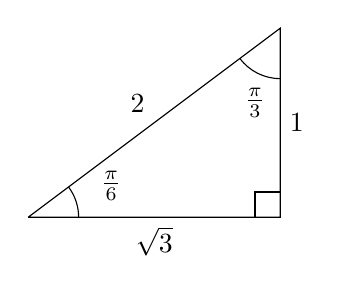
\begin{tikzpicture}[scale=0.8]
	  \draw[-] (0,0) -- node[below] {$\sqrt{3}$} ++(4,0) -- node[right] {$1$} ++ (0,3) -- node[above left] {$2$} ++(-4,-3);
		\draw[-] (4,0) -- (4-0.4,0) -- (4-0.4,0.4) -- (4,0.4) -- cycle;
		\draw (0.8,0) arc (0:36.86:0.8); \node[right] at (1,0.5) {$\frac{\pi}{6}$}; 
		\draw (4,3-0.8) arc (270:180+36.86:0.8); \node[below] at (3.6,2.2) {$\frac{\pi}{3}$}; 
\end{tikzpicture}
\end{center}
\end{Exercise}
\begin{Answer}[ref=\ExerciseLabel]
\multicolq[4]{
\Question $\frac{\pi}{6}$
\Question $-\frac{5\pi}{6}$
\Question $\frac{2\pi}{3}$
\Question $-\frac{\pi}{3}$
}
\end{Answer}

\begin{Exercise}[label={\thesubsection.\the\value{Exercise}}]
Plot  all complex numbers $z$ satisfying $\Arg{z} = -\frac{\pi}{2}$ in the complex plane.
\end{Exercise}

\begin{Exercise}[label={\thesubsection.\the\value{Exercise}}]
Plot all complex numbers $z$ satisfying $\Arg{z} \leq \frac{\pi}{2}$ and $|z|<2$ in the complex plane. 
\end{Exercise}

\begin{Exercise}[label={\thesubsection.\the\value{Exercise}}]
Write the following complex numbers in polar form.
\begin{align*}
\sqrt{3}-i &&1+\sqrt{3}i
\end{align*}
(Use the special triangle from exercise above). 
\end{Exercise}
\begin{Answer}[ref=\ExerciseLabel]
\multicolq[2]{
\Question $2\left(\cos\left(-\frac{\pi}{6}\right)+ i\sin\left(-\frac{\pi}{6}\right)\right)$
\Question $2\left(\cos\left(\frac{\pi}{3}\right)+ i\sin\left(\frac{\pi}{3}\right)\right)$
}
\end{Answer}

\begin{Exercise}[label={\thesubsection.\the\value{Exercise}}]
Write the following complex numbers in polar form.
\multicolq[4]{
\Question $2+i$
\Question $3+4i$
\Question $5$
\Question $6i$
}
\end{Exercise}
\begin{Answer}[ref=\ExerciseLabel]
\multicolq[2]{
\Question $2.236 \left(\cos\left(0.464 \right)+ i\sin\left(0.464 \right)\right)$
\Question $5\left(\cos\left( 0.927\right)+ i\sin\left( 0.927\right)\right)$
\Question $5\left(\cos\left(0 \right)+ i\sin\left(0 \right)\right)$
\Question $6\left(\cos\left( \frac{\pi}{2}\right)+ i\sin\left( \frac{\pi}{2}\right)\right)$
}
\end{Answer}
%</sec:comppolar>

\subsection{Exponential Form}

%<*sec:compexponential>
\begin{Exercise}[label={\thesubsection.\the\value{Exercise}}]
Write $ e^{3+i}$ and $e^{2-2i}$  in the form $a+ib$ (specify $a$ and $b$ to 2 decimal places).
\end{Exercise}
\begin{Answer}[ref=\ExerciseLabel]
$ 10.85 + 16.90 i $ and $ -3.07 - 6.72 i$ 
\end{Answer}


\begin{Exercise}[label={\thesubsection.\the\value{Exercise}}]
Write $1+i$ and $i$ in exponential form.
\end{Exercise}
\begin{Answer}[ref=\ExerciseLabel]
$\sqrt{2} e^{i \frac{\pi}{4}}$ and $ e^{i \frac{\pi}{2}}$.
\end{Answer}

\begin{Exercise}[label={\thesubsection.\the\value{Exercise}}]
Use the result of the previous question to work out
\begin{align*}
    (1+i)^2 && i(1+i) && \frac{i}{1+i} 
\end{align*}
using the exponential formulas, and verify your answers using complex arithmetic
\end{Exercise}
\begin{Answer}[ref=\ExerciseLabel]
$2 e^{i\frac{\pi}{2}}$, $\sqrt{2} e^{i\frac{3\pi}{4}}$, $\frac{1}{\sqrt{2}}e^{i\frac{\pi}{4}}$
\end{Answer}

\begin{Exercise}[label={\thesubsection.\the\value{Exercise}}]
Find the complex numbers $A,B$ such that
\begin{equation*}
    A e^{i\theta} + B e^{-i\theta} = 4 \cos(\theta) + 2 \sin(\theta).
\end{equation*}
\end{Exercise}
\begin{Answer}[ref=\ExerciseLabel]
$A=2-i$ and $B=2+i$
\end{Answer}

\begin{Exercise}[label={\thesubsection.\the\value{Exercise}}]
Given $\theta>0$, show that $y(t) = C e^{i\theta t} + D e^{-i\theta t}$ is a solution of $y''=-\theta^2 y$ and find $C, D$ such that $y(0)=0$ and $y'(0)=\theta$.
\end{Exercise}
\begin{Answer}[ref=\ExerciseLabel]
$C=-\frac{i}{2}$, $D=\frac{i}{2}$.
\end{Answer}

\begin{Exercise}[label={\thesubsection.\the\value{Exercise}}]
Show that
\begin{equation*}
        \tan(\theta) = i \left(\frac{1-e^{i2\theta}}{1+e^{i2\theta}}\right) = -i \left(\frac{1-e^{-i2\theta}}{1+e^{-i2\theta}}\right).
\end{equation*}
\end{Exercise}
%</sec:compexponential>

\subsection{De Moivre's Theorem}

%<*sec:compdmt>
\begin{Exercise}[label={\thesubsection.\the\value{Exercise}}]
Express $(2\left(\cos\left(\frac{\pi}{7}\right)+ i\sin\left(\frac{\pi}{7}\right)\right)^{6}$ in the form $a+ib$.
\end{Exercise}
\begin{Answer}[ref=\ExerciseLabel]
$2^6\cos\left(\frac{6\pi}{7}\right)+i2^6\sin\left(\frac{6\pi}{7}\right)$
\end{Answer}

\begin{Exercise}[label={\thesubsection.\the\value{Exercise}}]
 Use De Moivre's theorem to write $ (\sqrt{3} -i)^{4}$ and $(-1-i)^{25}$ in the form $a+ib$.
\end{Exercise}
\begin{Answer}[ref=\ExerciseLabel]
$-8-i 8\sqrt{3}$, $-4096 - 4096i$
\end{Answer}

\begin{Exercise}[label={\thesubsection.\the\value{Exercise}}] Use De Moivre's theorem to prove the identities
\Question $\sin(4\theta)=4(\sin(\theta)\cos^3(\theta) -\sin^3(\theta) \cos(\theta))$
\Question $\cos(5\theta)=\cos^5(\theta)-10\cos^3(\theta)\sin^2(\theta)+5\cos(\theta) \sin^4(\theta)$
\end{Exercise}


\begin{Exercise}[label={\thesubsection.\the\value{Exercise}}]
Find $4i$ in exponential form and then find its square roots.
\end{Exercise}
\begin{Answer}[ref=\ExerciseLabel]
Exponential form:$4 e^{i\frac{\pi}{2}}$
Square roots: $2 e^{i\frac{\pi}{4}}, 2 e^{i\frac{5\pi}{4}}$
\end{Answer}


\begin{Exercise}[label={\thesubsection.\the\value{Exercise}}]
Find all of the 4th roots of $1$ in exponential and $a+ib$ form.
\end{Exercise}
\begin{Answer}[ref=\ExerciseLabel]
Exponential form: $e^{i0}, e^{i\frac{\pi}{2}}, e^{i\pi}, e^{-i\frac{\pi}{2}}$.  
Cartesian form: $1,i,-1,-i$
\end{Answer}

\begin{Exercise}[label={\thesubsection.\the\value{Exercise}}]
Find all of the 3rd roots of $8$ in exponential and $a+ib$ form.
\end{Exercise}
\begin{Answer}[ref=\ExerciseLabel]
Exponential form: $2 e^{i0},2 e^{i\frac{2\pi}{3}},2 e^{-i\frac{2\pi}{3}}$. 
Cartesian form: $2,-1+i\sqrt{3},-1-i\sqrt{3}$
\end{Answer}
%</sec:compdmt>

\section{Matrices}

\subsection{Definitions}

(No tutorial exercises for this section)

\subsection{Matrix Operations}

%<*sec:matop>
\begin{Exercise}[label={\thesubsection.\the\value{Exercise}}]
Evaluate the following:  
\multicolq[2]{
\Question $\begin{pmatrix} 2&3\\ 1&4\\ -3&-2 \end{pmatrix} + \begin{pmatrix} 1&2\\ 3&5\\ 7&4 \end{pmatrix}$
\Question $\begin{pmatrix} 7&3&5\\ 8&4&6 \end{pmatrix}-\begin{pmatrix} 1&2&3\\ 4&6&5 \end{pmatrix}$
\Question $3 \begin{pmatrix} 2&3\\ 1&4\\ -3&-2 \end{pmatrix}$
\Question $\begin{pmatrix}2&3&5\\ 1&4&7 \end{pmatrix} 4$
\Question $5 \begin{pmatrix} 1&2\\ 3&4 \end{pmatrix}-3\begin{pmatrix}2&3\\ 4&5\end{pmatrix}
$
}
\end{Exercise} 
\begin{Answer}[ref=\ExerciseLabel] 
\multicolq[3]{
\Question $\begin{pmatrix}3&5\\4&9\\4&2\end{pmatrix}$
\Question $\begin{pmatrix}6&1&2\\4&-2&1\end{pmatrix}$
\Question $\begin{pmatrix}6&9\\3&12\\-9&-6\end{pmatrix}$
\Question $\begin{pmatrix}8&12&20\\4&16&28\end{pmatrix}$
\Question $\begin{pmatrix}-1&1\\3&5\end{pmatrix}$ 
}
\end{Answer}

\begin{Exercise}[label={\thesubsection.\the\value{Exercise}}]
Given:
\begin{align*}
A&=\begin{pmatrix}0&4&2\\-1&1&3\\2&0&-2\end{pmatrix} &
B&= \begin{pmatrix} 1&-3& 5\\2&0&-4\\3&2&0 \end{pmatrix}
\end{align*}
Find
\multicolq{
\Question $A+B$
\Question $A-B$
\Question $2A+3B$.
}
\end{Exercise} 
\begin{Answer}[ref=\ExerciseLabel] 
\multicolq{
\Question $\begin{pmatrix}1&1&7\\1&1&-1\\5&2&-2\end{pmatrix}$
\Question $\begin{pmatrix}-1&7&-3\\-3&1&7\\-1&-2&-2\end{pmatrix}$
\Question $\begin{pmatrix}3&-1&19\\4&2&-6\\13&6&-4\end{pmatrix}$
}
\end{Answer}

\begin{Exercise}[label={\thesubsection.\the\value{Exercise}}]
Given
\begin{align*}
A&= \begin{pmatrix} 2&0\\ 3&-1\\ -5&3\\ 1&4 \end{pmatrix}&
B&= \begin{pmatrix}-1&1\\ 0&3\\ 3&0\\ 0&1 \end{pmatrix}&
C&= \begin{pmatrix} 0&1\\ -1&1 \end{pmatrix}&
D&= \begin{pmatrix}0&1&3\\ -1&0&2\end{pmatrix}&
E&= \begin{pmatrix}1&0\\ -1&-2\end{pmatrix}
\end{align*}
Find the following sums or state that it does not exist:
\multicolq[5]{
\Question $2A+3B$
\Question $A+C$
\Question $B+D$
\Question $4C+2E$
\Question $D+E$
}
\end{Exercise}
\begin{Answer}[ref=\ExerciseLabel] 
\multicolq{
\Question $\begin{pmatrix}1&3\\6&7\\-1&6\\2&11\end{pmatrix}$ 
\Question does not exist
\Question does not exist 
\Question $\begin{pmatrix}2&4\\-6&0\end{pmatrix}$
\Question does not exist
}
\end{Answer}

\begin{Exercise}[label={\thesubsection.\the\value{Exercise}}]
Obtain $x,y, z$ and $w$ if
$\begin{pmatrix} -4x-4&2y-2\\ x+1&y-2\end{pmatrix}$
+
$\begin{pmatrix} 2x+2&-y\\y-1&x+1\end{pmatrix}$
=
$\begin{pmatrix}y-1&-z-3\\w&0\end{pmatrix}$
\end{Exercise} 
\begin{Answer}[ref=\ExerciseLabel] 
$x = -2, y = 3, z = -4, w = 1$
\end{Answer}
%</sec:matop>

\subsection{Matrix Multiplication}

%<*sec:matmult>
\begin{Exercise}[label={\thesubsection.\the\value{Exercise}}]
Evaluate the following:
\multicolq[4]{
\Question $\begin{pmatrix}1&2\end{pmatrix}\begin{pmatrix}-3\\ 4 \end{pmatrix}$
\Question $\begin{pmatrix}1&2&3\end{pmatrix}\begin{pmatrix}1\\2\\3\end{pmatrix}$
\Question $\begin{pmatrix}1&2\end{pmatrix}\begin{pmatrix}-3& 1\\4&2\end{pmatrix}$
\Question $\begin{pmatrix}1&2&3\end{pmatrix}\begin{pmatrix} 1& 3&-1\\2&3&-2\\3&-1&2\end{pmatrix}$
}
\end{Exercise} 
\begin{Answer}[ref=\ExerciseLabel] 
\multicolq[4]{
\Question $5$
\Question $14$
\Question $\begin{pmatrix}5&5\end{pmatrix}$ 
\Question $\begin{pmatrix}14& 6& 1\end{pmatrix}$
}
\end{Answer}

\begin{Exercise}[label={\thesubsection.\the\value{Exercise}}]
Given
\begin{align*}
A&=\begin{pmatrix}0&4&\ 2\\-1&1&3\\2&0&-2\end{pmatrix}&
B&=\begin{pmatrix}1&-3&5\\2&0&-4\\3&2&0\end{pmatrix}
\end{align*}
Evaluate
\multicolq{
\Question $AB$
\Question $BA$
\Question $B^2=BB$
}
\end{Exercise} 
\begin{Answer}[ref=\ExerciseLabel] 
\multicolq{
\Question $\begin{pmatrix}14&4&-16\\10&9&-9\\-4&-10&10\end{pmatrix}$
\Question $\begin{pmatrix}13&1&-17\\-8&8&12\\-2&14&12\end{pmatrix}$
\Question $\begin{pmatrix}10&7&17\\-10&-14&10\\7&-9&7\end{pmatrix}$
}
\end{Answer}

\begin{Exercise}[label={\thesubsection.\the\value{Exercise}}]
Given
\begin{align*}
E&=\begin{pmatrix}1&-1&1\\2&0&1\end{pmatrix}&
F&=\begin{pmatrix}1&-1&0\\0&1&-1\\1&1&1\end{pmatrix}&
G&=\begin{pmatrix}1&0\\0&1\\1&1\end{pmatrix}
\end{align*}
Verify that \ $(EF)G=E(FG)$.
\end{Exercise}

\begin{Exercise}[label={\thesubsection.\the\value{Exercise}}]
Evaluate the following products:
\multicolq[2]{
\Question $\begin{pmatrix}2&1&-1\end{pmatrix}
\begin{pmatrix}4&-1&2\\-1&0&1\\2&0&1\end{pmatrix}
\begin{pmatrix}2\\1\\-1\end{pmatrix}$
\Question $\begin{pmatrix}a&0&0\\0&b&0\\0&0&c\end{pmatrix}
\begin{pmatrix}x&0&0\\0&y&0\\0&0&z\end{pmatrix}$
}
\end{Exercise} 
\begin{Answer}[ref=\ExerciseLabel] 
\multicolq[2]{
\Question $4$
\Question $\begin{pmatrix}ax&0&0\\0&by&0\\0&0&cz\end{pmatrix}$
}
\end{Answer}

\begin{Exercise}[label={\thesubsection.\the\value{Exercise}}]
Matrices $A$,\ $B$ are said to commute if $AB=BA$.
\Question Prove that if $A$ and $B$ commute then they are square matrices of the same order.
\Question If 
$\begin{pmatrix}x&y\\3&1\end{pmatrix}$
commutes with 
$\begin{pmatrix}4&1\\3&0\end{pmatrix}$
Find $x$ and $y$.
\end{Exercise} 
\begin{Answer}[ref=\ExerciseLabel] 
$5,1$
\end{Answer}

\begin{Exercise}[label={\thesubsection.\the\value{Exercise}}]
Square matrix $A$ is said to be symmetric if $A^T=A$ and square matrix $B$ is said to be antisymmetric if $B^T=-B$.

Given the square matrix $R$, prove that $A=R+R^T$ is symmetric and $B=R-R^T$ is antisymmetric. You might need to use the result $(P+Q)^T=P^T+Q^T$ for matrices $P,Q$.

Show that any square matrix can be expressed as a sum of a symmetric matrix and an antisymmetric matrix.

Express in this way the matrix 
\begin{equation*}
\begin{pmatrix}1&2&4\\4&3&6\\6&2&5\end{pmatrix}
\end{equation*}
\end{Exercise}
\begin{Answer}[ref=\ExerciseLabel] 
\begin{align*}
A&=\frac{1}{2}(A+A^T)+\frac{1}{2}(A-A^T) && 
\begin{pmatrix}1&3&5\\3&3&4\\5&4&5\end{pmatrix}
+
\begin{pmatrix}0&-1&-1\\1&0&2\\1&-2&0\end{pmatrix}
\end{align*}
\end{Answer}

\begin{Exercise}[label={\thesubsection.\the\value{Exercise}}]
Verify the result $(AB)^T=B^TA^T$ when
\begin{align*}
A&=\begin{pmatrix}3&1&4\\1&2&0\\2&5&1\end{pmatrix}&
B&=\begin{pmatrix}6&5&1\\0&7&4\\8&1&3\end{pmatrix}
\end{align*}
\end{Exercise}

\begin{Exercise}[label={\thesubsection.\the\value{Exercise}}]
Given
\begin{align*}
A&=\begin{pmatrix}1&0&1\\1&2&0\end{pmatrix}&
B&=\begin{pmatrix}1&2&5\\3&1&2\\4&0&1\end{pmatrix}&
C&=\begin{pmatrix}3&2\\0&3\\1&1\end{pmatrix}
\end{align*}
Find $ABC$ and $C^TB^TA^T$.

\end{Exercise} 
\begin{Answer}[ref=\ExerciseLabel]
\multicolq[2]{
\Question $\begin{pmatrix}21&22\\30&35\end{pmatrix}$
\Question $\begin{pmatrix}21&30\\22&35\end{pmatrix}$
}
\end{Answer}
%</sec:matmult>

\subsection{Linear System of Equations} 

(No tutorial questions for this section)

\subsection{Solving Systems of Linear Equations} 

%<*sec:matlinsys>
\begin{Exercise}[label={\thesubsection.\the\value{Exercise}}]
Use the augmented matrix and elementary row operations to solve the following equations:
\begin{align*}
x + 2y &= 5&x + y &= 3.
\end{align*}
\end{Exercise}
\begin{Answer}[ref=\ExerciseLabel] 
 $x=1$, $y=2$
\end{Answer}

\begin{Exercise}[label={\thesubsection.\the\value{Exercise}}]
Use the augmented matrix and elementary row operations to solve the following sets of equations:
\multicolq[2]{
\Question 
\begin{align*}
x+y+z&=0\\
2x+4y+z&=1\\
3x+3y+z&=2
\end{align*}

\Question\begin{align*}
4u+2v-w&=0\\
5u+3v-w&=2\\
3u-v+4w&=2
\end{align*}
}
\end{Exercise}
\begin{Answer}[ref=\ExerciseLabel] 
\multicolq[2]{
\Question $x=1,y=0,z=-1$
\Question $x=-1,y=3,z=2$
}
\end{Answer}

\begin{Exercise}[label={\thesubsection.\the\value{Exercise}}]
The concentration $y(t)$ of a chemical in a solution is known to change with time $t$ seconds according to the formula
\begin{equation*}
         y(t) = a + b e^{-t}
\end{equation*}
but $a$ and $b$ are unknown. 
We have two experimental measurements $y(0) = 6$ and $y(2) = 3$ moles per litre.
Write down the linear system of equations for unknowns $a,b$ and solve it using elementary row operations.
\end{Exercise} 
\begin{Answer}[ref=\ExerciseLabel] 
\begin{align*}
a &= \frac{3-6e^{-2}}{1-e^{-2}} \approx 2.5304 & b &= \frac{3}{1-e^{-2}} \approx 3.4696
\end{align*}
\end{Answer}

\begin{Exercise}[label={\thesubsection.\the\value{Exercise}}]
Consider the distillation column example. Use the augmented matrix and elementary row operations to solve the system of linear equations there. Work to 3 decimal places.
\end{Exercise}
\begin{Answer}[ref=\ExerciseLabel]
(See lecture notes)
\end{Answer}

\begin{Exercise}[label={\thesubsection.\the\value{Exercise}}]
The voltages in a circuit calculation are found to satisfy
\begin{align*}
V_1 - V_3 &= 10, & V_2+V_1 &= 5, & 2V_3 + V_2 &= -3.
\end{align*}
Write the problem in matrix vector form and use the augmented matrix and elementary row operations to find the unknown voltages.
\end{Exercise} 
\begin{Answer}[ref=\ExerciseLabel] 
$\vv{V} = (12,-7,2)^T$
\end{Answer}
%</sec:matlinsys>

\subsection{Determinant of a Matrix} 

%<*sec:matdet>
\begin{Exercise}[label={\thesubsection.\the\value{Exercise}}]
Evaluate $\det\begin{pmatrix}2&3\\4&5\end{pmatrix}$ and 
$\begin{vmatrix}7&4\\5&2\end{vmatrix}$.
\end{Exercise} 
\begin{Answer}[ref=\ExerciseLabel] 
$-2$,$-6$
\end{Answer}

\begin{Exercise}[label={\thesubsection.\the\value{Exercise}}]
Let $F=\begin{pmatrix}-2&1&3\\4&-3&5\\-1&2&1\end{pmatrix}$.
Find the minors $M_{31}$ and $M_{23}$. Evaluate $\det(F)$ by expanding along the first row. Check your answer by expanding down the second column.
\end{Exercise} 
\begin{Answer}[ref=\ExerciseLabel] 
$14$,$-3$, $32$
\end{Answer}

\begin{Exercise}[label={\thesubsection.\the\value{Exercise}}]
Evaluate the determinants of the following matrices
\multicolq{
\Question $\begin{pmatrix}1&1&2\\2&1&1\\1&2&1\end{pmatrix}$
\Question $\begin{pmatrix}1&2&3\\3&1&2\\2&3&1\end{pmatrix}$
\Question $\begin{pmatrix}2&2&1\\-1&0&-1\\3&-1&3\end{pmatrix}$
}
\end{Exercise}
\begin{Answer}[ref=\ExerciseLabel] 
\multicolq{
\Question $4$
\Question $18$
\Question $-1$
}
\end{Answer}

\begin{Exercise}[label={\thesubsection.\the\value{Exercise}}]
Solve the equations:
\multicolq[2]{
\Question $\text{det}\begin{pmatrix}x&2&1\\-1&2&1\\1&0&1\end{pmatrix}=0$
\Question $\text{det}\begin{pmatrix}x^2&x&1\\4&2&1\\9&-3&1\end{pmatrix}=0$
}
\end{Exercise} 
\begin{Answer}[ref=\ExerciseLabel] 
\multicolq[2]{
\Question $x=-1$
\Question $x=2,-3$
}
\end{Answer}
%</sec:matdet>

\subsection{The Inverse of a Matrix}

%<*sec:matinv>
\begin{Exercise}[label={\thesubsection.\the\value{Exercise}}]
Given
\begin{align*}
A&=\begin{pmatrix}1&2\\1&1\end{pmatrix}&
B&=\begin{pmatrix}3&2\\5&3\end{pmatrix}
\end{align*}
\Question Calculate $A^{-1}$ and $B^{-1}$.
\Question Find the product $AB$ and calculate directly its inverse,  $(AB)^{-1}$.
\Question Find the product $B^{-1}A^{-1}$ and verify the result that $(AB)^{-1}=B^{-1}A^{-1}$.
\end{Exercise} 
\begin{Answer}[ref=\ExerciseLabel] 
\multicolq[2]{
\Question $\begin{pmatrix}-1&2\\1&-1\end{pmatrix}, \begin{pmatrix}-3&2\\5&-3\end{pmatrix}$
\Question $\begin{pmatrix}5&-8\\-8&13\end{pmatrix}$
\Question $\begin{pmatrix}5&-8\\-8&13\end{pmatrix}$
}
\end{Answer}

\begin{Exercise}[label={\thesubsection.\the\value{Exercise}}]
For the following rotation matrix:
$R_{xy}(\theta) = \begin{pmatrix} \cos(\theta) & \sin(\theta) & 0\\-\sin(\theta) & \cos(\theta) & 0\\  0 & 0 & 1 \end{pmatrix}$

Show that $R_{xy}(0) = I$, the identity matrix. Find the inverse of
$R_{xy}(\theta)$ for any real value of $\theta$. 
Verify that it is the indeed the inverse matrix by multiplying the two matrices together using the general matrix product method.
\end{Exercise} 
\begin{Answer}[ref=\ExerciseLabel] 
$R_{xy}^{-1}(\theta) = R_{xy}(-\theta)$.
\end{Answer}

\begin{Exercise}[label={\thesubsection.\the\value{Exercise}}]
Use the method of the inverse matrix to solve the following set of equations:
\begin{align*}
x+2y&=5 &x+y&=3
\end{align*}
\end{Exercise} 
\begin{Answer}[ref=\ExerciseLabel] 
$x=1, y=2$
\end{Answer}
%</sec:matinv>